{\large \textbf{- Άρτιες και περιττές συναρτήσεις}}
\vspace{1em}

Μια συνάρτηση $f: A \to \mathbb{R}$ λέγεται \textbf{άρτια} όταν ισχύει
\[
f(-x) = f(x) \quad \text{για κάθε } x, -x \in A.
\]

\vspace{1em}

Μια συνάρτηση $f: A \to \mathbb{R}$ λέγεται \textbf{περιττή} όταν ισχύει
\[
f(-x) = -f(x) \quad \text{για κάθε } x, -x \in A.
\]

\vspace{1em}

\textbf{Παρατηρήσεις:}
\begin{itemize}
  \item Για να έχει νόημα να εξετάσουμε αν μια συνάρτηση είναι άρτια ή περιττή, το πεδίο ορισμού $A$ πρέπει να είναι \textbf{συμμετρικό} ως προς το $0$, δηλαδή:
  \[
  x \in A \implies -x \in A.
  \]
  \item Γραφικά:
  \begin{itemize}
    \item Μια άρτια συνάρτηση έχει \textbf{άξονα συμμετρίας τον άξονα $y$}.
    \item Μια περιττή συνάρτηση έχει \textbf{κέντρο συμμετρίας την αρχή $O(0,0)$}.
  \end{itemize}
  \item Παραδείγματα:
  \[
  f(x) = x^2 \quad \text{(άρτια)}, \qquad g(x) = x^3 \quad \text{(περιττή)}.
  \]
  \item Καμία συνάρτηση δεν μπορεί να είναι ταυτόχρονα άρτια και περιττή, εκτός από τη μηδενι\-κή $f(x)=0$.
\end{itemize}

\textbf{Γραφικές Παραστάσεις:}

\begin{center}
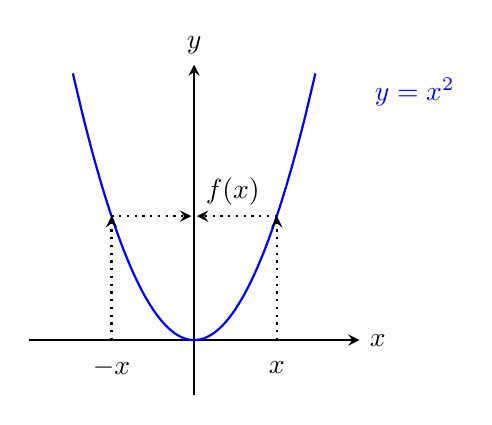
\begin{tikzpicture}[scale=0.7,  >=stealth]
  % Άξονες
  \draw[->, thick] (-3,0) -- (3,0) node[right] {$x$};
  \draw[->, thick] (0,-1) -- (0,5) node[above] {$y$};

  % Καμπύλη y = x^2
  \draw[domain=-2.2:2.2, smooth, variable=\x, blue, thick] plot ({\x}, {\x*\x});

  % Ετικέτα
  \node[blue] at (4,4.5) {$y=x^2$};
  \node at (1.5,-0.5) {$x$};
  \node at (-1.5,-0.5) {$-x$};
  \draw[dotted, thick, ->] (1.5, 0) -- (1.5, 2.25);
  \draw[dotted, thick, ->] (-1.5, 0) -- (-1.5, 2.25);
  \draw[dotted, thick, ->] (-1.5, 2.25) -- (-0.05, 2.25);
  \draw[dotted, thick, ->] (1.5, 2.25) -- (0.05, 2.25);
  \node at (0.7, 2.7) {$f(x)$};

\end{tikzpicture}
\hspace{2cm}
\begin{tikzpicture}[scale=0.7, >=stealth]
  % Άξονες
  \draw[->] (-3,0) -- (3,0) node[right] {$x$};
  \draw[->] (0,-3) -- (0,3) node[above] {$y$};

  % Καμπύλη y = x^3
  \draw[domain=-2:2, smooth, variable=\x, red, thick] plot ({\x}, {\x*\x*\x/2.8});

  % Ετικέτα
  \node[red] at (4,2.7) {$y=x^3$};

  \draw[dotted, thick, ->] (1.6, 0) -- (1.6, 1.46);
  \draw[dotted, thick, ->] (-1.6, 0) -- (-1.6, -1.46);
  \node at (-1.6,0.4) {$-x$};
  \node at (1.6,-0.4) {$x$};
  \draw[dotted, thick, ->] (-1.6, -1.46) -- (0, -1.46);
  \draw[dotted, thick, ->] (1.6, 1.46) -- (0, 1.46);
  \node at (0.85,-1.46) {$f(-x)$};
  \node at (-0.7,1.46) {$f(x)$};

\end{tikzpicture}
\end{center}
